\documentclass{article}
\usepackage{amsmath}

\begin{document}
\section{Gradient Descent}

\begin{align}
    \frac{dC(w_i)}{dw_i} = \lim_{\epsilon \to 0}\frac{C(w_i + \epsilon) - C(w_i)}{\epsilon}
\end{align}

\subsection{``Twice''}

\begin{align}
    C(w) &= \frac{1}{n} \sum_{i=1}^{n} (x_i w - y_i)^2 \\
    C'(w) 
	&= \left(\frac{1}{n} \sum_{i=1}^{n} (x_i w - y_i)^2\right)' \\
	&= \frac{1}{n}\left(\sum_{i=1}^{n} (x_i w - y_i)^2\right)' \\
	&= \frac{1}{n}\left((x_0 w - y_0)^2 + (x_1 w - y_1)^2 + (x_2 w - y_2)^2 + \hdots \right)' \\
	&= \frac{1}{n}\sum_{i=1}^{n} \left((x_i w - y_i)^2\right)' \\
	&= \frac{1}{n}\sum_{i=1}^{n} 2\left(x_i w - y_i) (x_i w - y_i\right)' \\
	&= \frac{1}{n}\sum_{i=1}^{n} 2\left(x_i w - y_i) ((x_i w)' - (y_i)'\right) \\
	&= \frac{1}{n}\sum_{i=1}^{n} 2\left(x_i w - y_i) (x_i w \right)' \\
	&= \frac{1}{n}\sum_{i=1}^{n} 2\left(x_i w - y_i\right)x_i \\
\end{align}

\begin{align}
	C(w) &= \frac{1}{n} \sum_{i=1}^{n} (x_i w - y_i)^2 \\
	C'(w) &= \frac{1}{n}\sum_{i=1}^{n} 2\left(x_i w - y_i\right)x_i \\
\end{align}

\subsection{One Neuron Model}

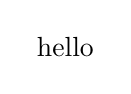
\begin{tikzpicture}
	\node at (0,0) {hello};
\end{tikzpicture}

\begin{align}
	y &= \sigma(xw + b) \\
	\sigma(x) &= \frac{1}{1 + e^{-x}} \\
	\sigma'(x) &= \sigma(x) (1-\sigma(x)) \\
\end{align}

\end{document}

